% !TEX root = ../../../prj4projektdokumentation.tex

\section{Modultest}

\subsection{Kontrolmodul}

\begin{center}
	\begin{tabular}{ | m{0.2\textwidth} | m{0.8\textwidth}|} 
		\hline
		\textbf{Test}					&Brugergrænsefladen modtager korrekte tal \\ \hline
		\textbf{Testbeskrivelse}		&Der testes at de værdiger, der kommer ind på Måleenheden er ens me værdigerne der vises på brugergrænsefladen. \\ \hline
		\textbf{Input}					&4VPP sinus på spænding indgang, 1VPP sinus på strøm indgang, 3,3ms forskydning \\ \hline
		\textbf{Forventet output}		&1,414V spænding, 0,354A strøm, 0,509 PF se figur \ref{fig:PFtest1}, 0 THD \\ \hline
		\textbf{Resultat}				&1,404V spænding, 0,359A strøm, 0,491, 0,2 THD,  se figur \ref*{fig:visningtest1} for resultat af skærm  \\ \hline
	\end{tabular}
\end{center}

\begin{figure}[H] % (alternativt [H])
	\centering
	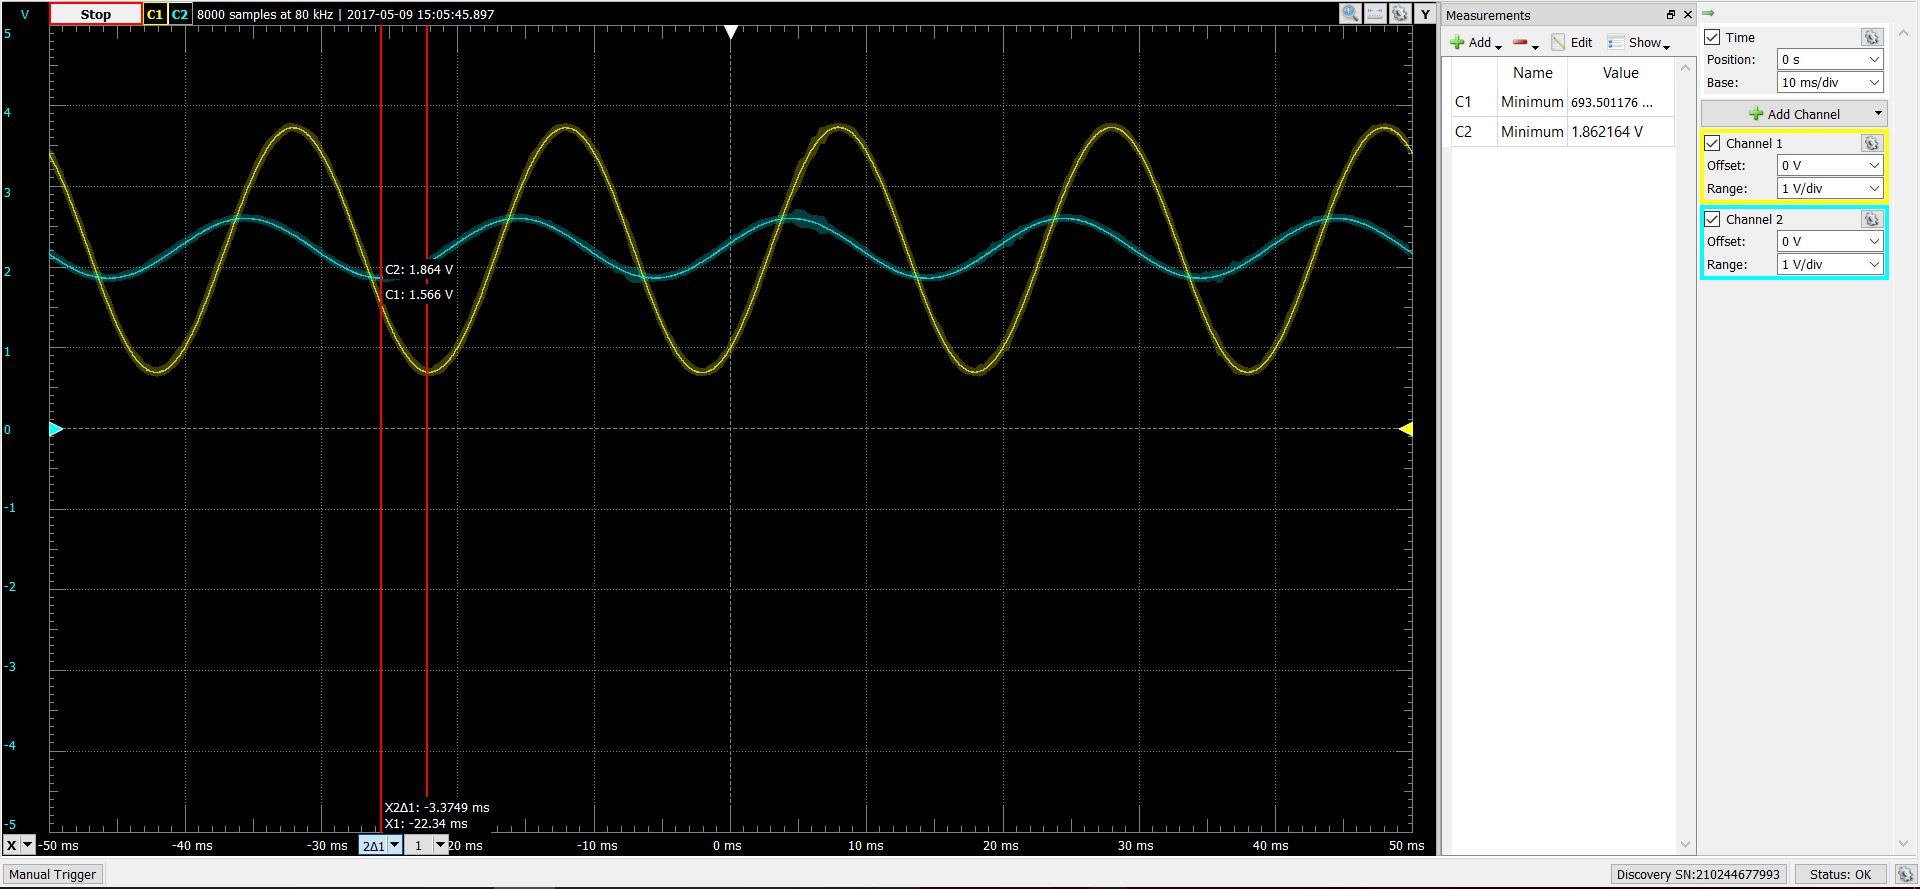
\includegraphics[width=0.7\textwidth]{Test/PFTest1}
	\caption{Visning af 3,3ms forsinkelse mellem strøm og spænding}
	\label{fig:PFtest1}
\end{figure}

\subsection{Brugergrænseflade}


\subsection{Kommunikationsmodul}